\subsection{环的整闭包. 整闭整环}

定义 3. 设 A 是环，R 是（交换）A-代数。由 R 中在 A 上为整的元素组成的 R 的子 A-代数 A'（第 1 节，命题 4 的推论 1）称为 A 在 R 中的整闭包。若 A' 等于 A 在 R 中的典范像，则称 A 在 R 中是整闭的。

\textbf{注}\par

\begin{enumerate}
\def\labelenumi{(\arabic{enumi})}
\item
  若 \(h: \mathbf{A} \to \mathbf{R}\) 是定义 \(\mathbf{R}\) 上 A-代数结构的环同态，则 \(\mathbf{A}\) 在 \(\mathbf{R}\) 中的整闭包也是 \(h(\mathbf{A})\) 在 \(\mathbf{R}\) 中的整闭包。另一方面，若 \(\mathbf{R}'\) 是 \(\mathbf{R}\) 的子代数，则 \(\mathbf{A}\) 在 \(\mathbf{R}'\) 中的整闭包是 \(\mathbf{A}' \cap \mathbf{R}'\) 。
\item
  若 A 是域，则 A 在 R 中的整闭包 \(A'\) 由 R 中在 A 上为代数的元素组成（第 1 节，例 1）；把域扩张所用的术语（《代数》，第 V 章，§3，第 3 节）加以推广，\(A'\) 这时也称为域 A 在代数 R 中的代数闭包，且若 \(A' = A\) ，称 A 在 R 中是代数闭的。
\end{enumerate}

定义 4. 若 A 是整环，则 A 在其分式域中的整闭包称为 A 的整闭包。若整环等于它的整闭包，则称它是整闭的。

\pandocbounded{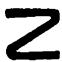
\includegraphics[keepaspectratio]{images/part002_6bc214f1.jpg}}

注意，整闭的整环未必在包含它的任何环中都是闭的，正如一个非代数闭的域这一例子所示。

命题 7. 设 A 是环，R 是 A-代数。A 在 R 中的整闭包 A' 是 R 中整闭的子环。

A' 在 R 中的整闭包由第 1 节命题 6 在 A 上是整的；因此它等于 A'。

推论. 整环 A 的整闭包是整闭的整环。

设 K 是 A 的分式域，B 是 A 的整闭包。显然

K 是 B 的分式域，只需把命题 7 应用于 R = K。

命题 8. 设 R 是环，\((\mathbf{B}_{\lambda})_{\lambda \in \mathbf{L}}\) 是 R 的子环族，且对每个 \(\lambda \in L\) ，设 \(A_{\lambda}\) 是 \(B_{\lambda}\) 的子环。若每个 \(A_{\lambda}\) 在 \(B_{\lambda}\) 中是整闭的，则 \(A = \bigcap_{\lambda \in L} A_{\lambda}\) 在 \(B = \bigcap_{\lambda \in L} B_{\lambda}\) 中是整闭的。

这由定义 3 及第 1 节命题 2 的推论 1 立即得出。

推论. 整环 A 的整闭子整环的非空族的每个交都是整闭的整环。

只需应用命题 8，取 R 与诸 \(B_{\lambda}\) 等于 A 的分式域 K，并注意 K 的在 K 中整闭的子环更是整闭的整环，因为其分式域含于 K。

命题 9. 设 A 是环，\((\mathbf{R}_i)_{1 \leqslant i \leqslant n}\) 是 A-代数的有限族，\(\mathbf{A}_i'\) 是 A 在 \(\mathbf{R}_i\) 中的整闭包（ \(1 \leqslant i \leqslant n\) ）。则 A 在 \(\mathbf{R} = \prod_{i=1}^{n} \mathbf{R}_i\) 中的整闭包等于 \(\prod_{i=1}^{n} \mathbf{A}_i'\) 。

这是第 1 节命题 3 的直接推论。

推论 1. 设 A 是既约 Noether 环，\(\mathfrak{p}_i\) （ \(1 \leqslant i \leqslant n\) ）是它的互异极小素理想，\(\mathbf{K}_i\) 是整环 \(\mathbf{A} / \mathfrak{p}_i\) 的分式域（典范同构于局部环 \(\mathbf{A}_{\mathfrak{p}_i}\) （第 IV 章，§2，第 5 节，命题 10）），\(\mathbf{A}_i'\) 是 A 在 \(\mathbf{K}_i\) 中的整闭包（ \(1 \leqslant i \leqslant n\) ）。则 A 的全分式环 B 到 \(\prod_{i=1}^{n} \mathbf{K}_i\) （出处同上）上的典范同构把 A 在 B 中的整闭包映到积环 \(\prod_{i=1}^{n} \mathbf{A}_i'\) 上。

推论 2. 要使既约 Noether 环在其分式环中是整闭的，必须且只需它是整闭（Noether）整环的直合成。

